% =============================================================================
% Capitulo 2 - Estado del arte
% =============================================================================
\chapter{Estado del arte}
\label{cap:estado_arte}

\section{Sistemas de detección de drones}
\label{sec:deteccion_drones}

La proliferación de drones comerciales de bajo coste ha provocado un crecimiento sostenido de incidentes en infraestructuras críticas durante la última década. El cierre del aeropuerto londinense de Gatwick en diciembre de 2018, la invasión del espacio aéreo de plantas nucleares francesas en 2019 o las múltiples incursiones detectadas sobre instalaciones militares europeas han convertido el llamado \emph{counter-UAS}  en un dominio tecnológico con producto comercial maduro y literatura académica abundante \cite{taha2022counteruav,shi2025airport}. Este capítulo revisa las principales familias tecnológicas empleadas para detectar drones, los sistemas comerciales más representativos de cada una y justifica la elección de la aproximación basada en radiofrecuencia adoptada en este TFG.

\subsection{Familias tecnológicas}
\label{subsec:familias_deteccion}

La detección de un dron se aborda habitualmente con cuatro tipos de sensores que explotan principios físicos distintos.

\textbf{Radar.} Los sistemas radar iluminan activamente el espacio con ondas electromagnéticas y analizan los ecos reflejados por el blanco. Son la solución tradicional en vigilancia aérea, pero los drones de pequeño tamaño  presentan una sección radar (RCS) muy reducida, lo que ha obligado a desarrollar radares específicos en banda K o Ka con escaneo electrónico. Funcionan en cualquier condición de iluminación y meteorología, pero son sistemas activos que emiten energía, requieren licencia y resultan costosos \cite{taha2022counteruav}.

\textbf{Acústica.} Los sensores acústicos detectan el ruido característico de los motores y hélices del dron mediante arrays de micrófonos y técnicas de \emph{beamforming}. Son pasivos, baratos y operan en condiciones de baja visibilidad, pero su alcance está fuertemente limitado por la atenuación del sonido en el aire y por el ruido de fondo urbano. Funcionan bien para clases pequeñas a corta distancia  y se han convertido en un componente recurrente de redes de bajo coste, como las desplegadas durante el conflicto de la guerra de Ucrania.

\textbf{Óptica.} Las cámaras visibles e infrarrojas confirman visualmente la presencia del dron y permiten su identificación. Son imprescindibles como capa de verificación final, pero por sí solas presentan limitaciones importantes: dependencia de iluminación, vulnerabilidad a la meteorología adversa, campos de visión estrechos y necesidad de saber dónde apuntar. En la práctica, se utilizan en arquitecturas \emph{slew-to-cue} guiadas por otro sensor primario \cite{shi2025airport}.

\textbf{Radiofrecuencia.} Los sistemas RF capturan de forma pasiva las comunicaciones entre el dron y su mando, o entre el dron y el satélite GNSS, y las clasifican por su firma espectral. Aprovechan que la mayoría de drones comerciales mantienen un enlace de mando, telemetría o vídeo activo durante toda la operación. Son completamente pasivos, no requieren licencia de emisión, y permiten detectar el dron incluso antes de que esté en línea de vista directa (NLOS), ya que la radio del piloto y la del dron son detectables por separado. Su limitación más conocida es la incapacidad para detectar drones controlados por fibra óptica o autónomos sin enlace, situación que ha cobrado relevancia operacional reciente \cite{taha2022counteruav}.

\subsection{Sistemas comerciales destacados}
\label{subsec:sistemas_comerciales}

Como referencia del estado de la técnica industrial, se describen brevemente los productos más representativos en cada familia tecnológica. La selección se ha realizado priorizando sistemas con documentación técnica pública y referencias en la literatura académica de \emph{counter-UAS}.

\textbf{DroneShield RfOne MKII.} Sensor estacionario de detección y radiogoniometría RF completamente pasivo, con cobertura de \ang{90} por unidad y capacidad de combinar cuatro sensores para alcanzar cobertura \ang{360}. Opera contra una base de datos propietaria de firmas RF actualizada por suscripción y permite triangulación cuando se despliegan varios sensores en red \cite{droneshield_rfone}.


\begin{figure}[H]
    \centering
    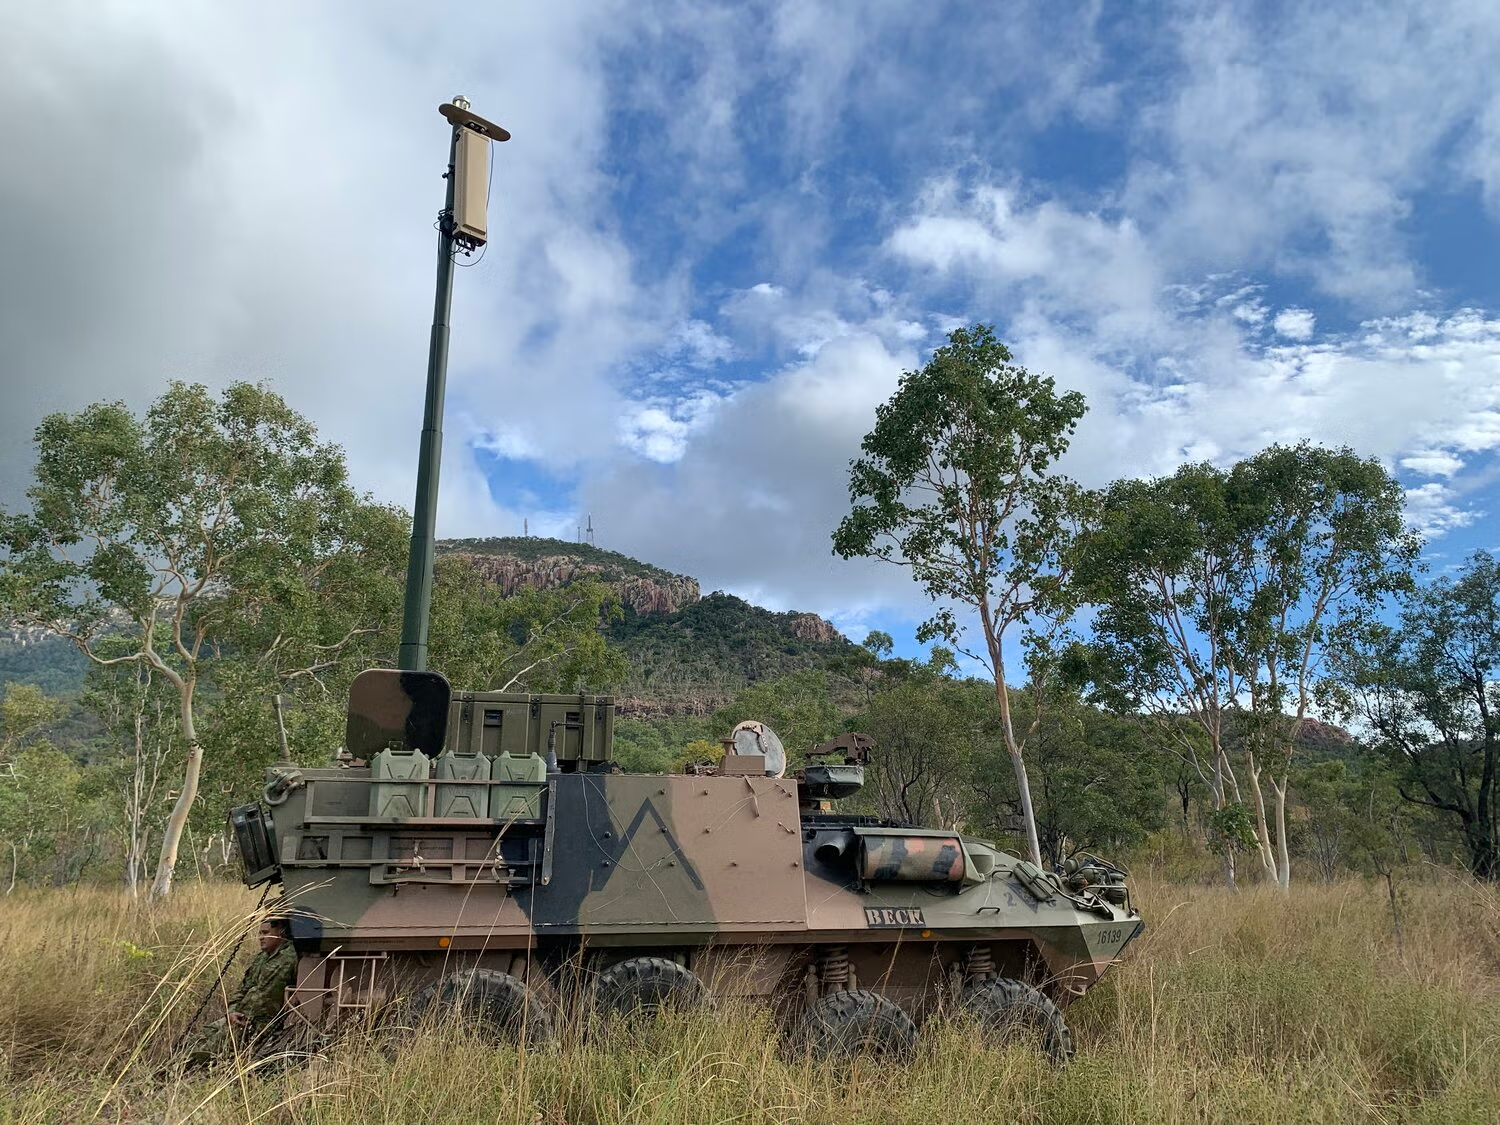
\includegraphics[width=0.6\textwidth]{figuras/estado del arte/Army2-6.png}
    \caption{Sensor estacionario de detección y radiogoniometría RF DroneShield RfOne MKII, desplegado para vigilancia de largo alcance. Fuente: DroneShield~\cite{droneshield_rfone}.}
    \label{fig:droneshield_rfone}
\end{figure}

\textbf{Aaronia AARTOS.} Plataforma modular construida en torno al analizador de espectro en tiempo real SPECTRAN V6, que ofrece hasta \SI{980}{\mega\hertz} de ancho de banda instantáneo en el rango \SIrange{10}{8000}{\mega\hertz}. Combinado con la antena IsoLOG 3D DF y la suite RTSA-Suite PRO, decodifica protocolos como DJI OcuSync y Mavlink y alcanza hasta \SI{50}{\kilo\meter} de rango de detección en configuraciones desplegadas \cite{aaronia_aartos}.

\begin{figure}[H]
    \centering
    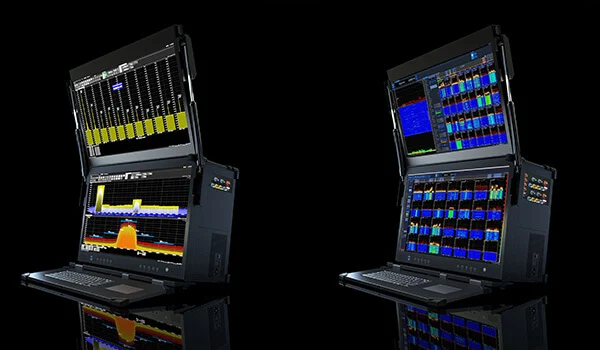
\includegraphics[width=0.6\textwidth]{figuras/estado del arte/aaronia.png}
    \caption{Sistema de detección de drones Aaronia AARTOS, construido en torno al analizador de espectro en tiempo real SPECTRAN V6 y la antena IsoLOG 3D DF. Fuente: Aaronia AG~\cite{aaronia_aartos}.}
    \label{fig:aaronia_aartos}
\end{figure}

\textbf{Dedrone RF-360.} Sensor RF pasivo en red, con grado de protección IP65 y conectividad LTE/GPS integrada para despliegue rápido. Integra varios SDR internos que clasifican el dron mediante la suite DroneTracker y permite localización por triangulación con alcance de hasta \SI{5}{\kilo\meter} en configuraciones direccionales \cite{dedrone_rf360}.


\begin{figure}[H]
    \centering
    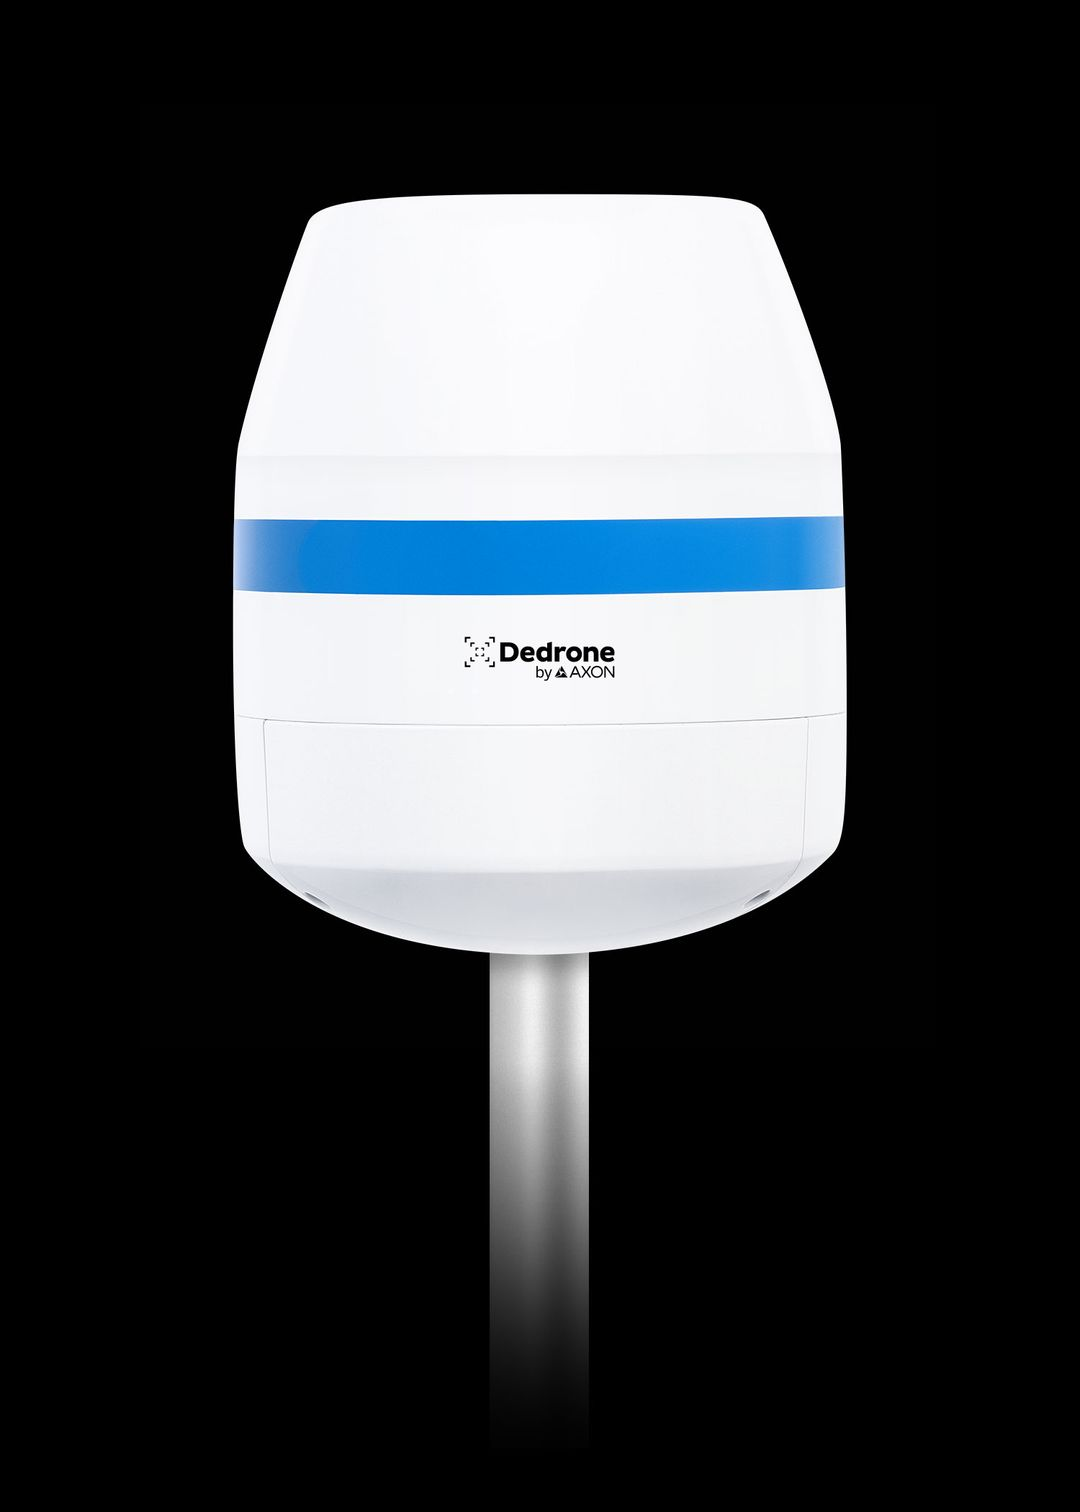
\includegraphics[width=0.6\textwidth]{figuras/estado del arte/dedrone.jpg}
    \caption{Sensor RF pasivo en red Dedrone RF-360, con grado de protección IP65 y conectividad LTE/GPS integrada para despliegue rápido. Fuente: Dedrone~\cite{dedrone_rf360}.}
    \label{fig:dedrone_rf360}
\end{figure}

\textbf{Rohde \& Schwarz ARDRONIS.} Sistema profesional de detección, clasificación y localización RF que cubre \SIrange{20}{6000}{\mega\hertz} con una única antena. Su característica más relevante para este TFG es el algoritmo de separación automática basada en perfiles, capaz de aislar la señal de un enlace FHSS concreto en escenarios con espectro densamente ocupado \cite{rohde_ardronis}.

\begin{figure}[H]
    \centering
    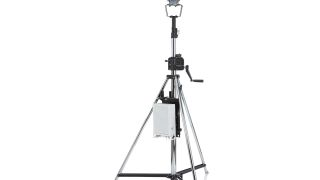
\includegraphics[width=0.6\textwidth]{figuras/estado del arte/ardronis.jpg}
    \caption{Sistema de detección, clasificación y localización RF Rohde \& Schwarz ARDRONIS, con algoritmo de separación automática de enlaces FHSS en espectro densamente ocupado. Fuente: Rohde \& Schwarz~\cite{rohde_ardronis}.}
    \label{fig:rohde_ardronis}
\end{figure}

\subsection{Comparativa y justificación de la elección RF}




La aproximación RF resulta especialmente adecuada para un TFG experimental por tres razones. En primer lugar, la captura es pasiva y se realiza con receptores SDR de coste moderado (HackRF, USRP, BladeRF), lo que evita los problemas regulatorios asociados a sensores activos. En segundo lugar, los drones comerciales mayoritarios mantienen su enlace de mando activo en bandas ISM bien delimitadas (\SI{2.4}{\giga\hertz} y \SI{5.8}{\giga\hertz}), lo que permite trabajar sobre datasets reproducibles y dispositivos accesibles como el DJI Mini 3. En tercer lugar, la representación tiempo-frecuencia de la señal RF habilita el uso de arquitecturas estándar de visión por computador, conectando el problema con un campo metodológicamente maduro \cite{rfuav2025,allahham2019dronerf}.

El principal riesgo de la aproximación RF es la presencia simultánea de WiFi y Bluetooth en la banda de \SI{2.4}{\giga\hertz}, que comparten morfología FHSS y OFDM con el enlace del dron y constituyen el reto técnico que motiva este trabajo. Las secciones siguientes profundizan en la caracterización RF del enlace del DJI Mini 3 (Sección~\ref{sec:comunicaciones_rf}), las representaciones tiempo-frecuencia empleadas (Sección~\ref{sec:representaciones_tf}) y los modelos de aprendizaje profundo aplicables al problema (Sección~\ref{sec:deep_rf}).


\section{Comunicaciones RF en drones comerciales}
\label{sec:comunicaciones_rf}

Para entender la dificultad de la detección RF de drones es necesario conocer qué señales conviven en la banda en la que estos operan y qué morfología presentan en un espectrograma. Esta sección describe brevemente el contexto de la banda \SI{2.4}{\giga\hertz}, los enlaces de control y vídeo más extendidos en drones comerciales, y las clases de señal que actúan habitualmente como interferencia.

\subsection{La banda ISM de 2,4~GHz}
\label{subsec:banda_ism}

La banda \emph{Industrial, Scientific and Medical} (ISM) de \SIrange{2400}{2483.5}{\mega\hertz} está disponible sin licencia en prácticamente todo el mundo. Como consecuencia, es compartida por una gran variedad de tecnologías inalámbricas, entre ellas WiFi (802.11\,b/g/n/ax), Bluetooth Classic y Bluetooth Low Energy, ZigBee, hornos microondas, sistemas de mando radioeléctrico para modelismo y la mayoría de enlaces de control de drones comerciales \cite{ieee80211_2020,bluetooth_core_5_4}. Esta coexistencia obliga a cualquier detector basado en RF a operar en un entorno crónicamente congestionado, donde la mera presencia de energía en la banda no es informativa.

WiFi ocupa canales de \SI{20}{\mega\hertz} (con bonding opcional a \SI{40}{\mega\hertz}) centrados a partir de \SI{2412}{\mega\hertz} con separación de \SI{5}{\mega\hertz}, lo que da hasta catorce canales solapados de los que solo tres (1, 6 y 11) son habitualmente utilizables sin colisión. Bluetooth Classic divide la banda en \num{79} canales de \SI{1}{\mega\hertz} y salta entre ellos a una tasa de \num{1600} saltos por segundo siguiendo una secuencia pseudoaleatoria.







\subsection{La plataforma DJI Mini 3 y el enlace OcuSync O2}
\label{sec:plataforma_mini3}

El dron empleado como fuente de señal en este trabajo es el DJI Mini 3. Su enlace de comunicación con el mando utiliza el sistema de transmisión de vídeo \emph{OcuSync O2} (comercializado por DJI como \emph{DJI O2}), el mismo que monta el DJI Mini 2; la variante DJI Mini 3 Pro emplea, en cambio, la generación posterior OcuSync O3~\cite{dji_mini3_manual,heliguy_dji_transmission}. El enlace opera en las bandas de \SIrange{2.4000}{2.4835}{\giga\hertz} y \SIrange{5.725}{5.850}{\giga\hertz}. Este trabajo se centra en la banda de \SI{2.4}{\giga\hertz}, donde el enlace coexiste con WiFi y Bluetooth.

La característica más relevante para la detección es que OcuSync emplea salto de frecuencia (FHSS) con selección adaptativa del canal: el sistema es capaz de elegir automáticamente el mejor canal de transmisión, evitando las zonas del espectro más congestionadas por otras señales. En la práctica, esto significa que las ráfagas del enlace tienden a situarse en los huecos libres entre los canales WiFi ocupados (típicamente los canales 1, 6 y 11), de forma análoga al salto de frecuencia adaptativo (AFH) del Bluetooth. Como consecuencia, en un espectrograma de la banda las transmisiones del dron aparecen como ráfagas estrechas y dispersas en frecuencia, en lugar de columnas anchas y fijas como las del WiFi.

Este comportamiento es lo que hace interesante el problema: la firma del dron no ocupa una posición fija del espectro, sino que se reparte dinámicamente por los huecos libres, compartiendo banda y morfología con otras señales de salto de frecuencia como el Bluetooth. Conviene además señalar que el propio DJI Mini 3 integra módulos WiFi y Bluetooth 5.2.








\subsection{Enlaces de control y vídeo de drones comerciales}
\label{subsec:enlaces_drones}

Los drones comerciales suelen mantener dos canales de comunicación activos durante el vuelo: un enlace de mando y telemetría hacia el dron, y un enlace de vídeo descendente. El sistema más extendido en el mercado de consumo es la familia OcuSync de DJI, que ha evolucionado desde Lightbridge (2014) hasta las generaciones actuales O3 y O4 \cite{heliguy_dji_transmission}. Todas las versiones de OcuSync emplean modulación OFDM para el vídeo y un mecanismo de salto en frecuencia (FHSS) para el mando, con anchos de banda configurables y operación dual en \SI{2.4}{\giga\hertz} y \SI{5.8}{\giga\hertz} \cite{schiller2023droneid}. Además, los drones DJI modernos emiten paquetes \emph{DroneID} para cumplir con normativas Remote-ID, con una estructura periódica de ráfagas cortas en el orden de centenares de microsegundos y anchos de banda de pocos megahercios \cite{schiller2023droneid,vainilavicius2024dji}.

Fuera del ecosistema DJI conviven otros sistemas RC abiertos. ExpressLRS (ELRS) es un protocolo de código abierto basado en transceptores Semtech (LoRa y FLRC) que opera en \SI{2.4}{\giga\hertz} y \num{868}/\SI{915}{\mega\hertz} \cite{expresslrs}. TBS Crossfire combina DSSS y FHSS en bandas sub-GHz \cite{tbs_crossfire}. Por último, los drones de bajo coste basados en WiFi-FPV (Parrot AR.Drone y similares) producen una firma indistinguible de una red WiFi convencional. Para el propósito de este TFG resulta especialmente relevante OcuSync, por ser el sistema utilizado en la mayoría de drones de consumo actuales.






\subsection{Comparativa morfológica de las señales en 2,4~GHz}
\label{subsec:comparativa_morfologia}

Desde el punto de vista de un espectrograma, las tres clases de señal más significativas en la banda presentan estructuras visualmente distinguibles. WiFi se manifiesta como columnas verticales anchas y persistentes coincidentes con los canales fijos. El enlace OFDM de vídeo de los drones aparece como una banda continua de anchura media. Bluetooth Classic y el enlace de mando FHSS de OcuSync producen ráfagas estrechas y dispersas, geométricamente similares entre sí, lo que constituye el principal reto del problema. La Figura~\ref{fig:espectrograma_interferencia} ilustra estas estructuras en una captura sin presencia de dron, y la Tabla~\ref{tab:morfologia_rf} resume las propiedades morfológicas de cada clase.

\begin{figure}[H]
\centering
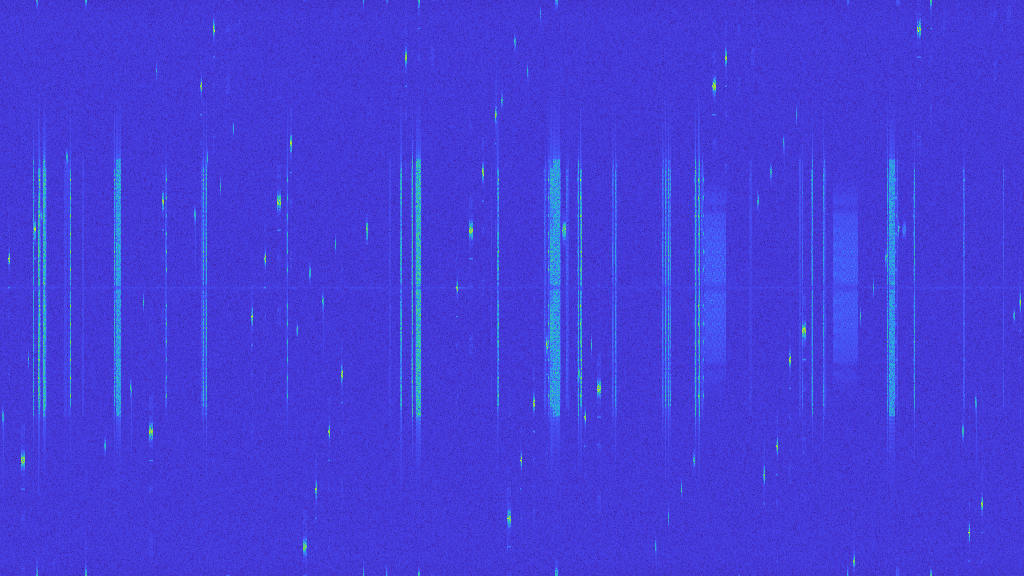
\includegraphics[width=0.95\textwidth]{figuras/estado del arte/mini3_nodrone_w2_s01_cap03__seg0068.png}
\caption{Ejemplo de espectrograma en la banda de \SI{2.4}{\giga\hertz} con interferencia WiFi y Bluetooth. Las columnas verticales anchas corresponden a canales WiFi ocupados; las ráfagas estrechas y dispersas son atribuibles a Bluetooth y a otros emisores ISM, y presentan una morfología parcialmente similar a la firma esperada del enlace de mando de un dron.}
\label{fig:espectrograma_interferencia}
\end{figure}

\begin{table}[H]
\centering
\caption{Comparativa morfológica de las señales presentes en la banda de \SI{2.4}{\giga\hertz}.}
\label{tab:morfologia_rf}
\begin{tabularx}{\textwidth}{lXXXX}
\toprule
\textbf{Propiedad} & \textbf{OcuSync (mando)} & \textbf{OcuSync (vídeo)} & \textbf{WiFi 802.11g/n} & \textbf{Bluetooth Classic} \\
\midrule
Técnica & FHSS & OFDM adaptativo & OFDM en canal fijo & FHSS \\
Ancho de banda & Estrecho por ráfaga & Medio/ancho continuo & Ancho, canal fijo & Muy estrecho por salto \\
Duración de actividad & Ráfagas cortas dispersas & Continua durante vídeo & Por tramas, ráfagas variables & Ráfagas muy cortas, periódicas \\
Posición en frecuencia & Variable & Centrada en canal libre & Canales fijos (1, 6, 11) & Distribuida por toda la banda \\
Apariencia espectral & Rectángulos pequeños dispersos & Banda continua bien definida & Columnas verticales anchas & Rectángulos pequeños dispersos \\
\bottomrule
\end{tabularx}
\end{table}

La similitud morfológica entre las ráfagas FHSS de Bluetooth y las del enlace de mando del dron es el motivo por el que la detección no puede basarse en simples descriptores espectrales agregados y motiva el uso de modelos de aprendizaje profundo capaces de aprender patrones tiempo-frecuencia más sutiles, como los descritos en las secciones siguientes.

\section{Representaciones tiempo-frecuencia de señales RF}
\label{sec:representaciones_tf}

La clasificación de señales de radiofrecuencia mediante aprendizaje profundo requiere transformar las muestras IQ del receptor en una representación bidimensional que la red pueda procesar como una imagen. La literatura ha explorado varias alternativas, todas ellas basadas en mostrar simultáneamente cómo se distribuye la energía de la señal en tiempo y en frecuencia \cite{cohen1995timefrequency,boashash2015timefrequency}.

El espectrograma derivado de la transformada de Fourier de tiempo corto (STFT) es la representación más extendida. Trabajos recientes sobre clasificación de drones por RF, como RFUAV \cite{rfuav2025} o DroneRF \cite{allahham2019dronerf}, lo emplean como entrada estándar a arquitecturas convolucionales preentrenadas, aprovechando que su formato matricial encaja directamente con redes diseñadas para imágenes naturales. Su popularidad se explica por tres factores: un coste computacional reducido, una buena estabilidad numérica y la compatibilidad inmediata con modelos como ResNet, VGG o EfficientNet sin necesidad de adaptaciones.

Otras representaciones aparecen ocasionalmente en la literatura. El escalograma, obtenido mediante la transformada wavelet continua (CWT), ofrece resolución adaptativa y resulta atractivo para señales con eventos transitorios de muy distintas duraciones \cite{mallat2008wavelet}. Las distribuciones cuadráticas como la de Wigner-Ville proporcionan una resolución conjunta tiempo-frecuencia superior a la STFT, pero introducen términos cruzados que dificultan su interpretación visual y su uso con redes convolucionales \cite{boashash2015timefrequency}. En el ámbito específico de la detección y clasificación RF de drones mediante aprendizaje profundo, el espectrograma STFT se ha consolidado como la representación de referencia.




\section{Aprendizaje profundo para detección y clasificación de señales RF}
\label{sec:deep_rf}

Las redes neuronales convolucionales han demostrado gran capacidad para extraer patrones espaciales en imágenes. Al convertir una señal RF en un espectrograma, la tarea puede tratarse como un problema de reconocimiento de patrones visuales, donde las estructuras relevantes son ráfagas, bandas, discontinuidades, densidad de ocupación o cambios de energía. Dentro de este marco, este trabajo emplea dos familias de arquitecturas con propósitos distintos: una red de clasificación de imágenes (ResNet) y una red de detección de objetos (YOLO).

\subsection{Redes convolucionales residuales: ResNet}
\label{subsec:resnet}

ResNet (\emph{Residual Network}) es una arquitectura convolucional introducida por He et~al. \cite{he2016resnet} que resolvió el problema de degradación que aparece al aumentar la profundidad de las redes. Su aportación clave son las \emph{conexiones residuales} o de salto, que suman la entrada de un bloque a su salida y permiten que el gradiente fluya directamente a través de la red. Gracias a ello es posible entrenar modelos de decenas o cientos de capas sin que el entrenamiento se degrade. La familia incluye variantes de distinta profundidad (ResNet18, 34, 50, 101, 152); la versión ResNet18, con aproximadamente once millones de parámetros, ofrece un buen compromiso entre capacidad y coste computacional.

Una característica determinante para este trabajo es la disponibilidad de pesos preentrenados sobre ImageNet, lo que permite aplicar \emph{transfer learning}: se reutiliza el extractor de características aprendido sobre imágenes naturales y se sustituye únicamente la capa final por una salida adaptada a las clases del problema. Esto reduce drásticamente la cantidad de datos y de tiempo de entrenamiento necesarios, algo especialmente valioso en un dataset RF de tamaño limitado.

En este TFG, ResNet18 se utiliza como clasificador de imagen completa: primero como detector binario \emph{drone}/\emph{interference} en un enfoque inicial, y posteriormente como segunda etapa del sistema, encargada de identificar el modelo concreto de dron a partir de la región o el espectrograma asociado a una detección.

\subsection{Detección de objetos en una etapa: YOLO}
\label{subsec:yolo}

A diferencia de la clasificación, que asigna una única etiqueta a la imagen completa, la \emph{detección de objetos} localiza y clasifica simultáneamente múltiples regiones dentro de la imagen mediante cajas delimitadoras (\emph{bounding boxes}). YOLO (\emph{You Only Look Once}), propuesto por Redmon et~al. \cite{redmon2016yolo}, fue uno de los primeros detectores de una sola etapa: en lugar de proponer regiones candidatas y clasificarlas después (enfoque en dos etapas, como R-CNN), plantea la detección como una única regresión sobre una rejilla que predice cajas y probabilidades de clase en una sola pasada. Esto le confiere una velocidad muy superior, apta para operación en tiempo real.

La versión empleada en este trabajo es YOLOv8, desarrollada por Ultralytics \cite{jocher2023yolov8}. Respecto a versiones anteriores incorpora un diseño \emph{anchor-free} (predice directamente la posición de las cajas sin anclas predefinidas), una cabeza de detección desacoplada y un \emph{backbone} convolucional optimizado, y se distribuye en variantes de distinto tamaño (n, s, m, l, x). La variante \emph{nano} (YOLOv8n), con unos tres millones de parámetros, es la más ligera. El rendimiento de estos detectores se mide habitualmente con la precisión media promedio (mAP) a distintos umbrales de solapamiento (IoU) entre las cajas predichas y las reales.

En este TFG, YOLOv8 constituye la primera etapa del sistema: en lugar de clasificar el espectrograma completo, detecta y localiza las ráfagas individuales dentro de él. Esta decisión es metodológicamente relevante, ya que al operar sobre regiones locales el modelo se ve obligado a atender a la morfología de las ráfagas y no al contexto global de la captura, evitando el sesgo que afectaba al enfoque de clasificación de imagen completa.

\subsection{Sistema en dos etapas y referencia RFUAV}
\label{subsec:two_stage_rfuav}

La combinación de ambas arquitecturas define un sistema en dos etapas: YOLO responde a la pregunta de presencia y localización , mientras que ResNet18 responde a la de identificación. Esta separación permite que cada red resuelva un problema acotado y más sencillo que el problema global.

El trabajo RFUAV constituye la referencia más cercana, ya que propone un conjunto de datos de señales RF de drones y una metodología basada en la conversión de datos IQ a espectrogramas para aplicar después modelos de aprendizaje profundo \cite{rfuav2025}. Este TFG toma esa idea general, pero la adapta a un caso experimental propio centrado en la detección de la firma del dron frente a interferencias WiFi/Bluetooth y en su posterior clasificación por modelos.



\section{Conclusiones del estado del arte}
\label{sec:conclusiones_estado_arte}

La revisión realizada muestra que la detección de drones mediante radiofrecuencia es una línea madura y activa. Las familias tecnológicas disponibles (óptica, acústica, radar y RF) presentan ventajas complementarias, pero los sistemas basados en RF destacan por su carácter pasivo, su capacidad de operar a largo alcance y su compatibilidad con receptores SDR de bajo coste, lo que los convierte en una opción especialmente atractiva para entornos experimentales y académicos.

El análisis de las comunicaciones empleadas por los drones comerciales revela que la banda de \SI{2.4}{\giga\hertz} es un escenario complejo en el que coexisten enlaces propietarios como OcuSync, redes WiFi, dispositivos Bluetooth y otras emisiones ISM. Esta coexistencia obliga a abordar el problema más allá de la simple detección de energía, ya que las firmas relevantes deben distinguirse en presencia de interferencias estructuralmente similares. Las representaciones tiempo-frecuencia, y en particular el espectrograma, se han consolidado en la literatura como entrada estándar para esta tarea, al hacer visibles patrones que en el dominio temporal resultan difíciles de separar.

Sobre esta representación, las arquitecturas de aprendizaje profundo basadas en redes convolucionales han demostrado un rendimiento sólido en problemas de clasificación de señales RF, apoyándose en datasets públicos cada vez más amplios. Sin embargo, gran parte de los trabajos existentes evalúan sus modelos en condiciones controladas o con interferencias limitadas, y un porcentaje reducido incorpora técnicas de interpretabilidad que permitan verificar que la red aprende características físicamente significativas y no artefactos del dataset.

De este recorrido se desprende que el problema sigue abierto en su vertiente más realista: la evaluación de detectores RF basados en aprendizaje profundo frente a escenarios con congestión espectral elevada y la validación, mediante herramientas de interpretabilidad, de que las decisiones del modelo se apoyan en la huella tiempo-frecuencia del enlace del dron. Este es el contexto en el que se enmarca el presente trabajo.